\documentclass{article}
\usepackage{tikz}
\usetikzlibrary{positioning}
\begin{document}
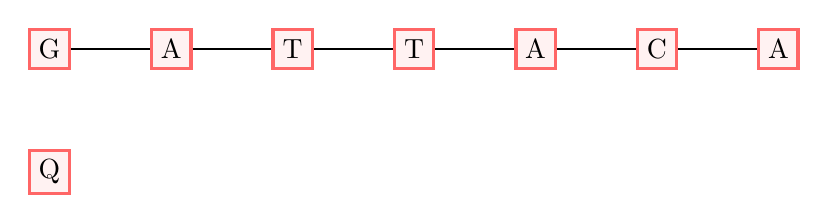
\begin{tikzpicture}[
roundnode/.style={circle, draw=green!60, fill=green!5, very thick, minimum size=7mm},
squarednode/.style={rectangle, draw=red!60, fill=red!5, very thick, minimum size=5mm},
]
%Nodes
\node[squarednode] (seqA1) {G};
\node[squarednode] (seqA2) [right=of seqA1] {A};
\node[squarednode] (seqA3) [right=of seqA2] {T};
\node[squarednode] (seqA4) [right=of seqA3] {T};
\node[squarednode] (seqA5) [right=of seqA4] {A};
\node[squarednode] (seqA6) [right=of seqA5] {C};
\node[squarednode] (seqA7) [right=of seqA6] {A};

\node[squarednode] (seqB1) [below=of seqA1] {Q};

%\node[roundnode]        (uppercircle)       [above=of seqA1] {1};
%\node[squarednode]      (rightsquare)       [below=of seqA1] {3};
%\node[roundnode]        (lowercircle)       [below=of seqA1] {4};

%Lines
\draw (seqA1) -- (seqA2);
\draw (seqA2) -- (seqA3);
\draw (seqA3) -- (seqA4);
\draw (seqA4) -- (seqA5);
\draw (seqA5) -- (seqA6);
\draw (seqA6) -- (seqA7);

%\draw[->] (uppercircle.south) -- (seq1.north);
%\draw[->] (seq1.east) -- (rightsquare.west);
%\draw[->] (rightsquare.south) .. controls +(down:7mm) and +(right:7mm) .. (lowercircle.east);
%\draw[->] (rightsquare.south) -- (lowercircle.east);
\end{tikzpicture}
\end{document}
